\lstinputlisting[language=bash,basicstyle=\small]{python_codes/fieldstone_77/keywords}

\begin{center}
Code at \url{https://github.com/cedrict/fieldstone/tree/master/python_codes/fieldstone_77}
\end{center}

\par\noindent\rule{\textwidth}{0.4pt}

%%%%%%%%%%%%%%%%%%%%%%%%%%%%%%%%%%%%%%%%%%%%%%%%%%%%%%%%%%%%%%%%%%%%%%%%%%%%%%%%%%%%%%%%%%%%

I have implemented the two variants of the Rannacher-Turek element presented
in Section~\ref{ss:RTq1p0}.
After communicating with Prof. Turek, I also implemented that Laplace 
formulation of the Stokes equation, i.e. we assume $\eta$ to be constant 
and therefore for an incompressible flow the momentum conservation 
equation becomes 
\[
-\vec\nabla p + \eta \Delta \vec\upnu = \vec{b}
\]
This yields a different form of the viscous block of the Stokes system
as explained in Section~\ref{ss:isovisc}.
I use an isoparametric mapping, but I have tried a $Q_1$ mapping and given that 
all elements are square it does not change anything. 
I have implemented to benchmark based on manufactured solutions:
\begin{itemize}
\item Donea-Huerta, see Section~\ref{mms1}

\begin{center}
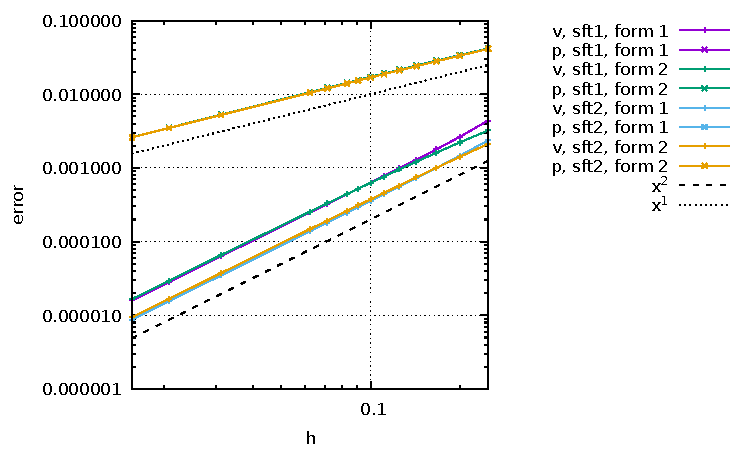
\includegraphics[width=7cm]{python_codes/fieldstone_77/results/dh/errors}
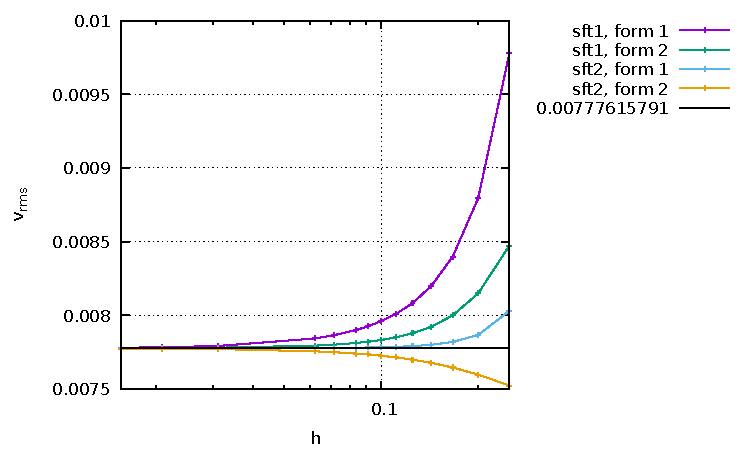
\includegraphics[width=7cm]{python_codes/fieldstone_77/results/dh/vrms}\\
{\captionfont Left: Velocity and pressure error convergence; Right: 
root mean square velocity}
\end{center}

\item Volker John benchmark, see Section~\ref{mms10}

\begin{center}
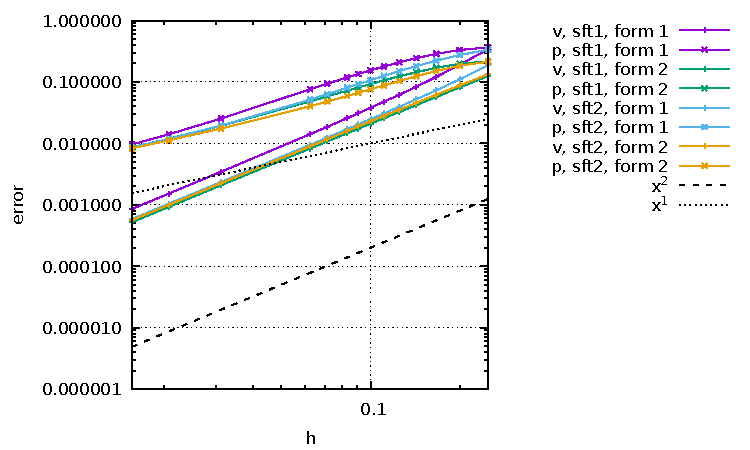
\includegraphics[width=7cm]{python_codes/fieldstone_77/results/vj/errors}
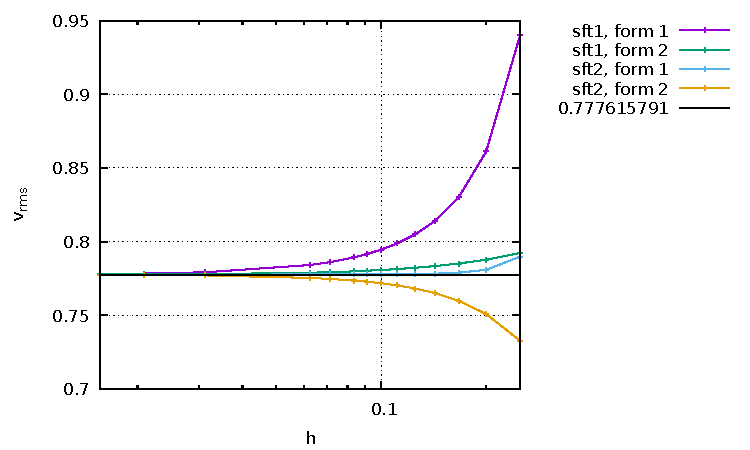
\includegraphics[width=7cm]{python_codes/fieldstone_77/results/vj/vrms}\\
{\captionfont Left: Velocity and pressure error convergence; Right: 
root mean square velocity}
\end{center}

\end{itemize}

We see that both variants of the element exhibit a quadratic convergence for the
velocity error and a linear convergence for the pressure error. Also the root mean square 
velocity measurements logically converge to their analytical values.  

Since this element has been thoroughly studied and proved to be LBB stable one could think that it 
should then replace the standard $Q_1 \times P_0$: near identical cost, but LBB stable and 
identical convergence!

However, there is no free lunch. I have also implemented another experiment: a unit cube domain
filled with a fluid of density $\rho=1$ and a cube of size $0.25\times 0.25$ centered in the domain
with density $\rho+\delta \rho$. Both fluids have the same viscosity $\eta=1$ for simplicity.
Boundary conditions are no slip on all sides, gravity points downwards with $|\vec{g}|=1$.

\noindent
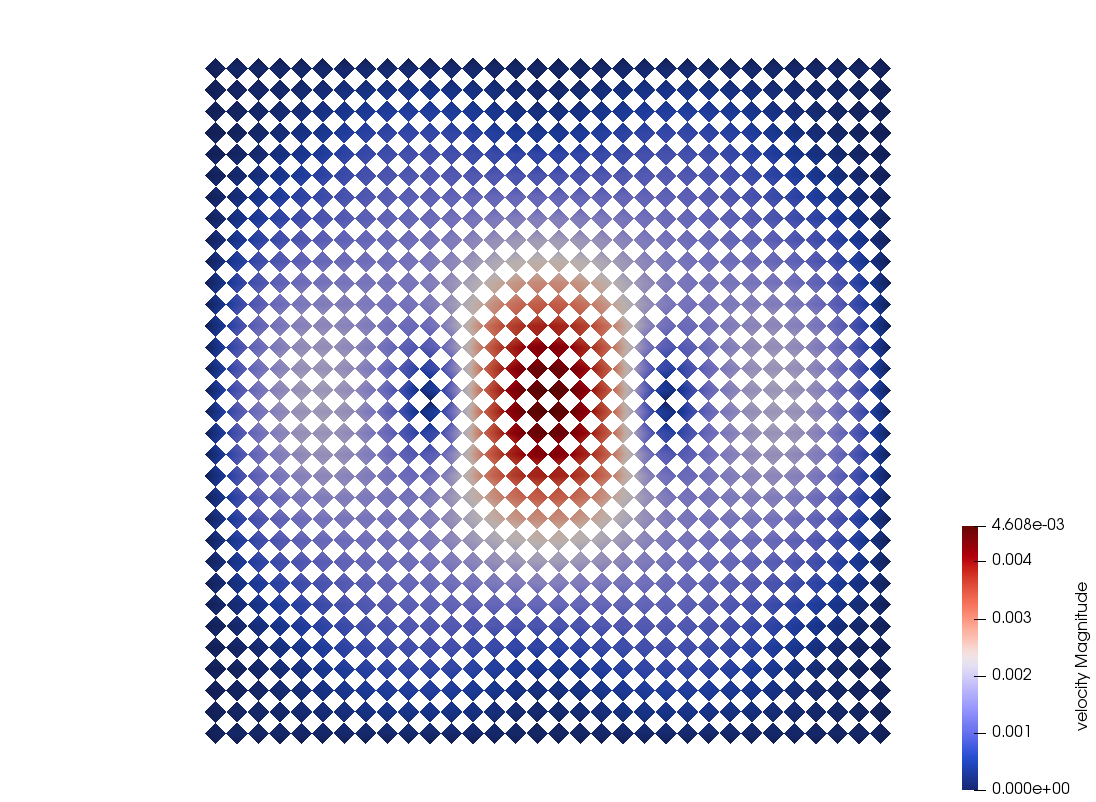
\includegraphics[width=4cm]{python_codes/fieldstone_77/results/block/velA}
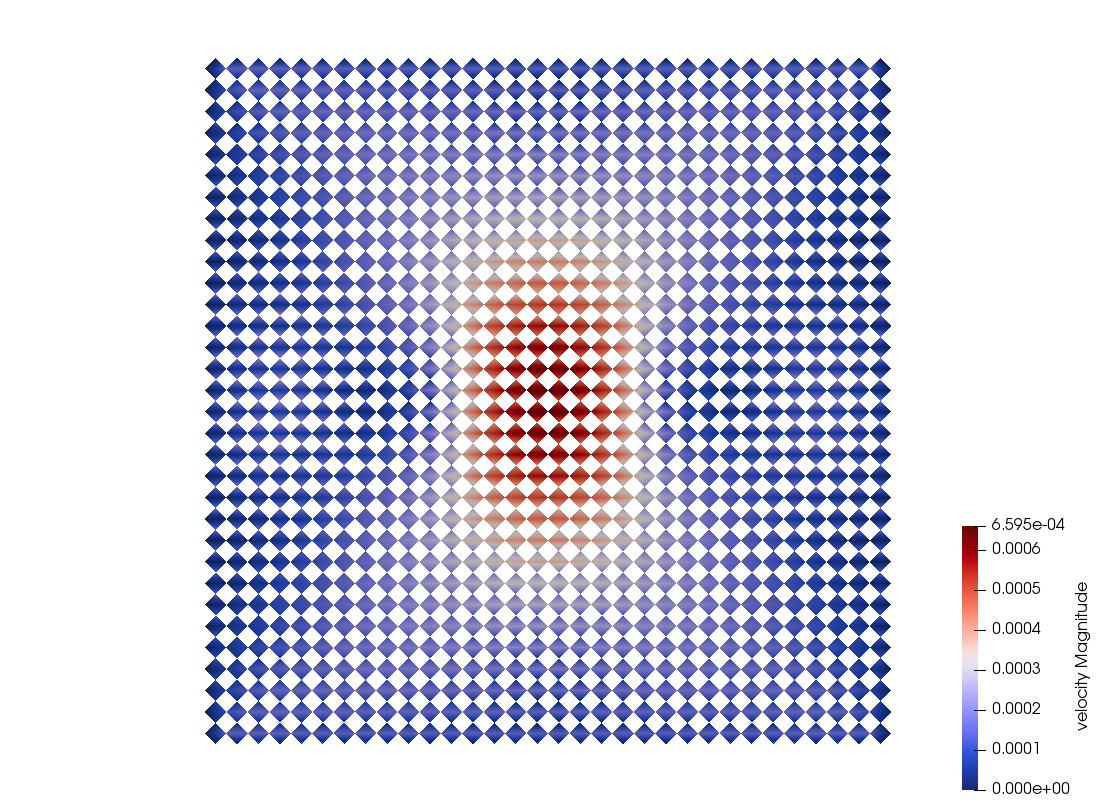
\includegraphics[width=4cm]{python_codes/fieldstone_77/results/block/velB}
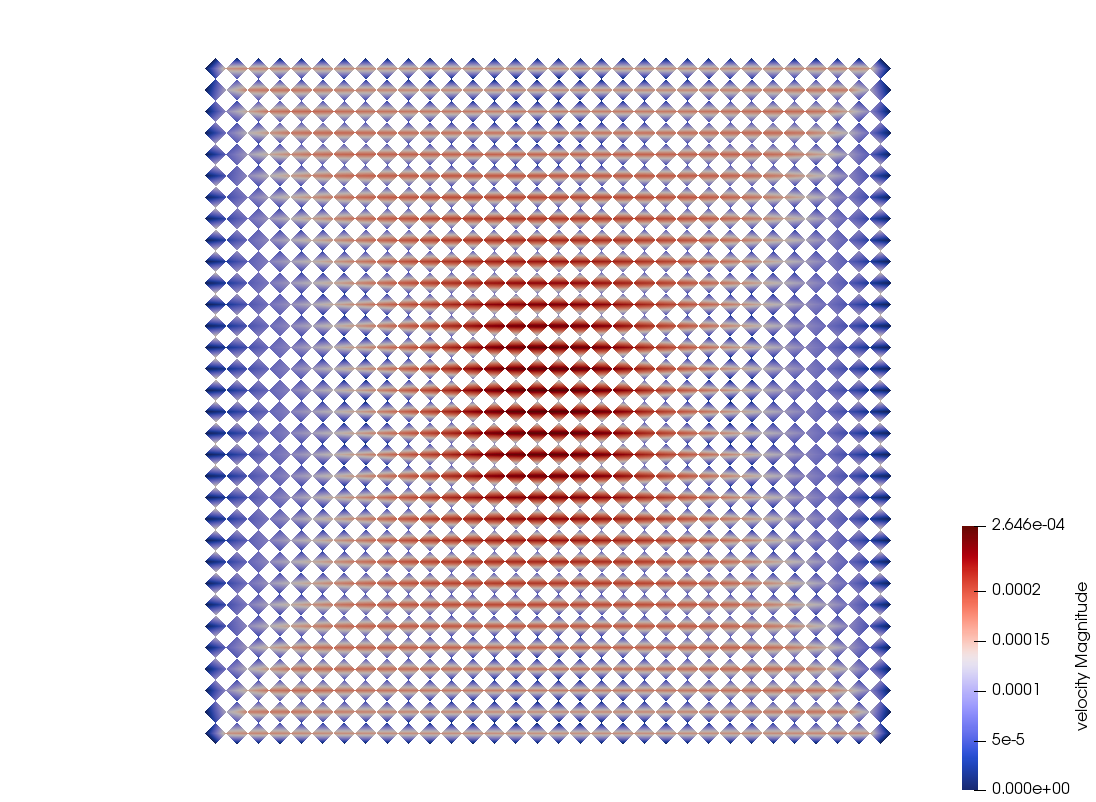
\includegraphics[width=4cm]{python_codes/fieldstone_77/results/block/velC}
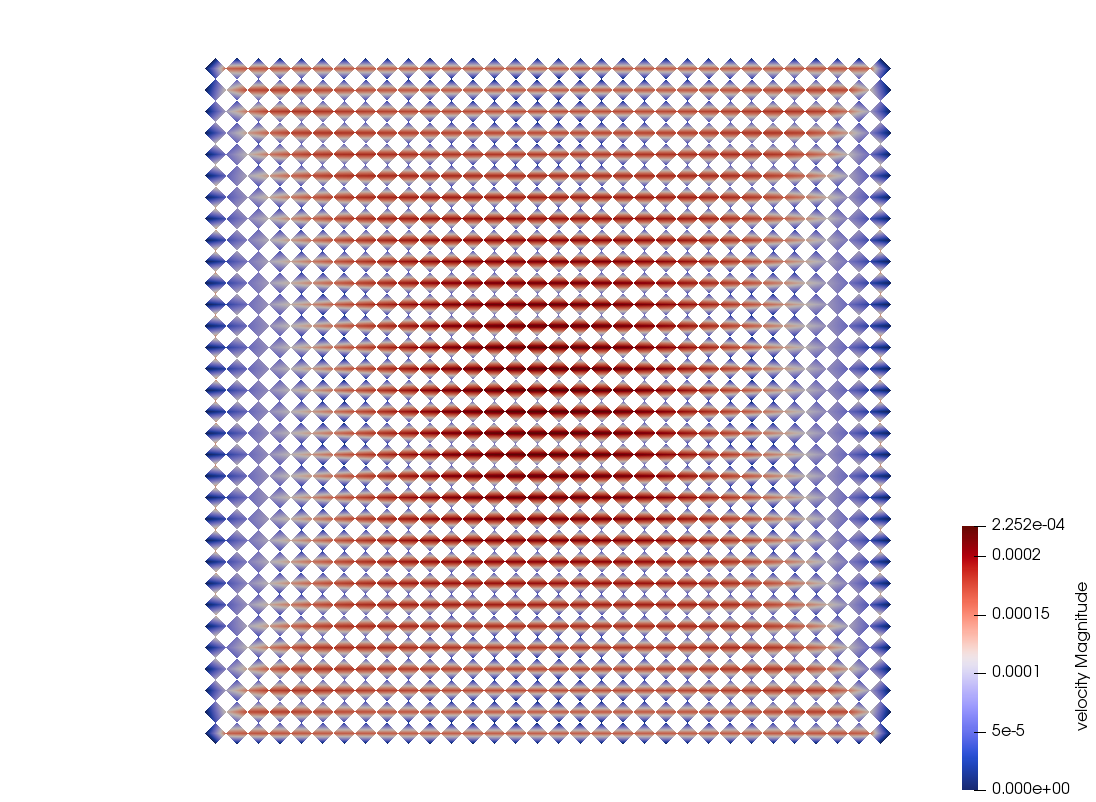
\includegraphics[width=4cm]{python_codes/fieldstone_77/results/block/velD}\\
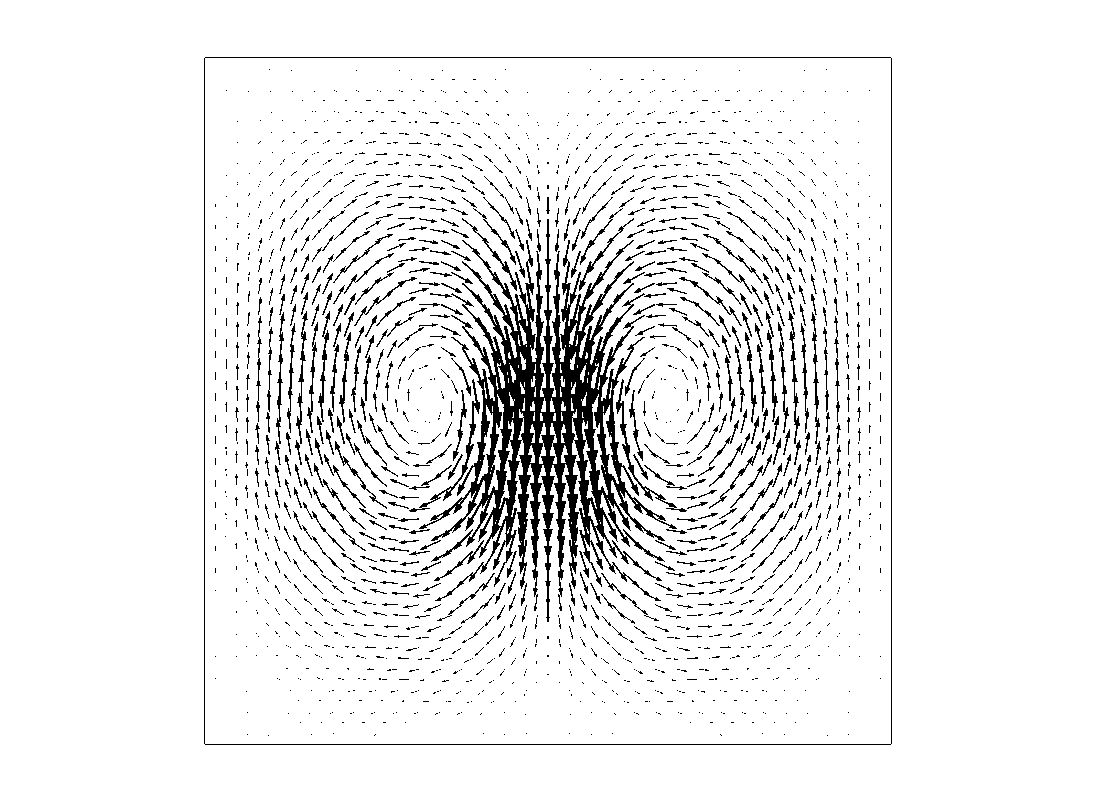
\includegraphics[width=4cm]{python_codes/fieldstone_77/results/block/velAv}
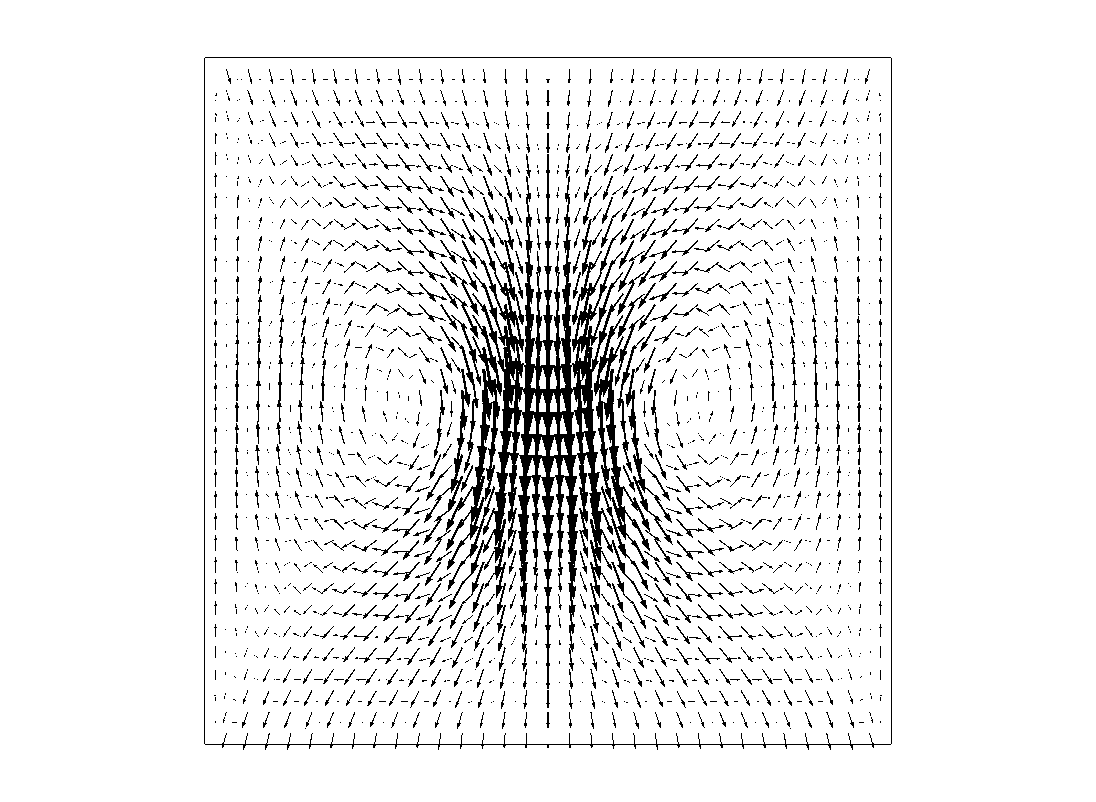
\includegraphics[width=4cm]{python_codes/fieldstone_77/results/block/velBv}
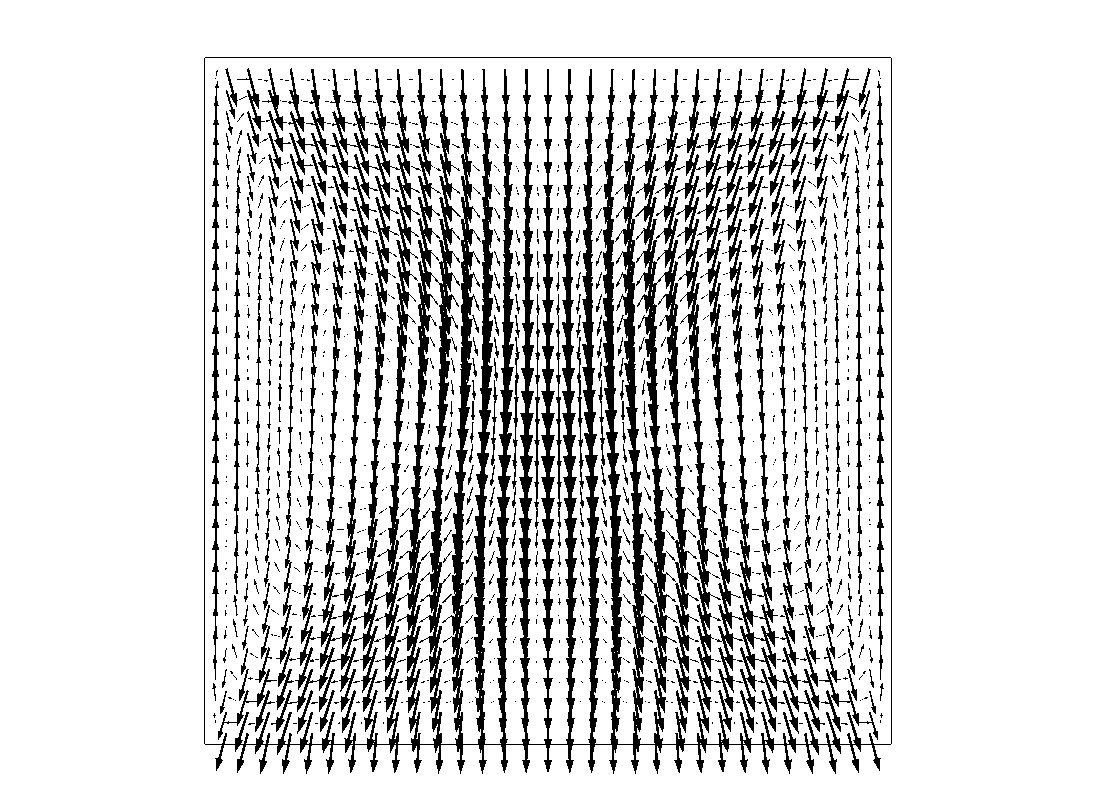
\includegraphics[width=4cm]{python_codes/fieldstone_77/results/block/velCv}
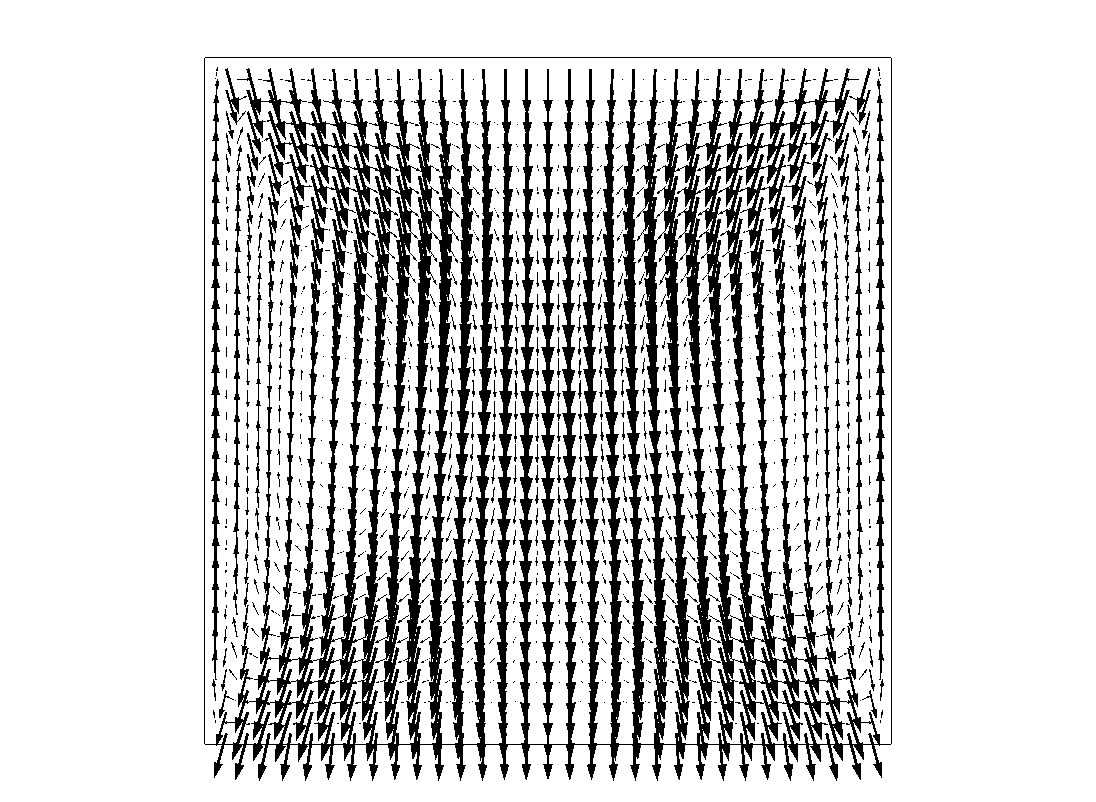
\includegraphics[width=4cm]{python_codes/fieldstone_77/results/block/velDv}\\
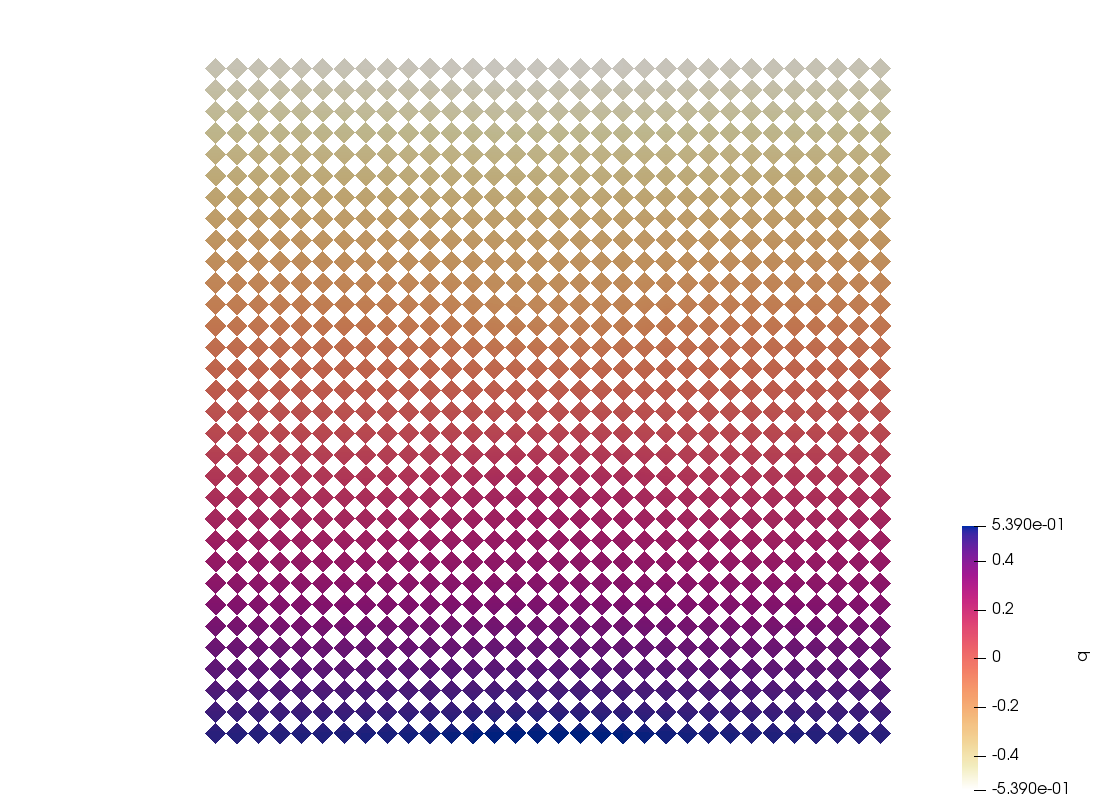
\includegraphics[width=4cm]{python_codes/fieldstone_77/results/block/pA}
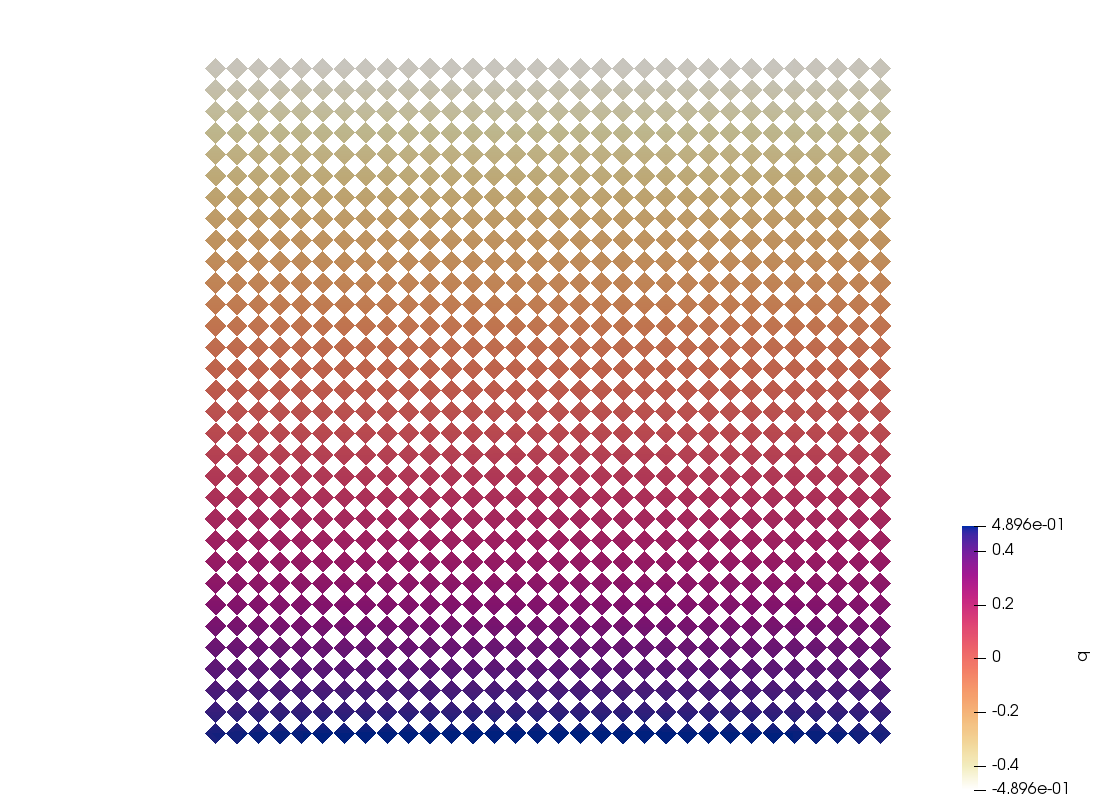
\includegraphics[width=4cm]{python_codes/fieldstone_77/results/block/pB}
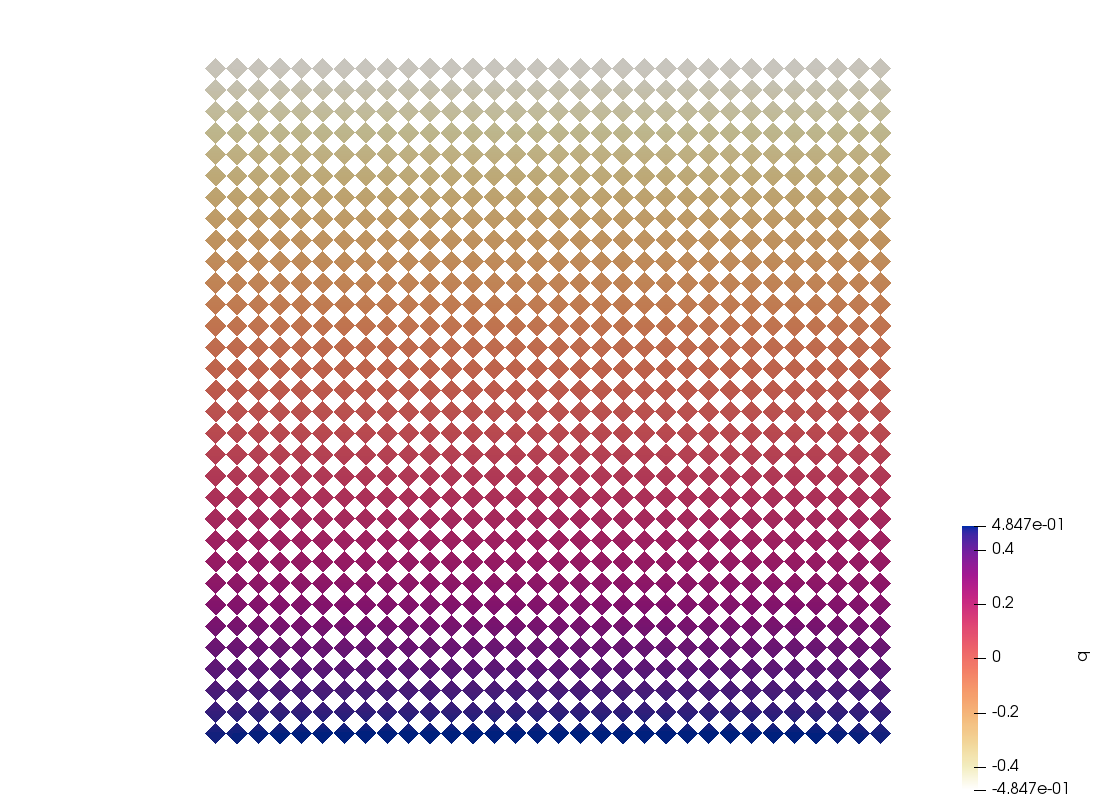
\includegraphics[width=4cm]{python_codes/fieldstone_77/results/block/pC}
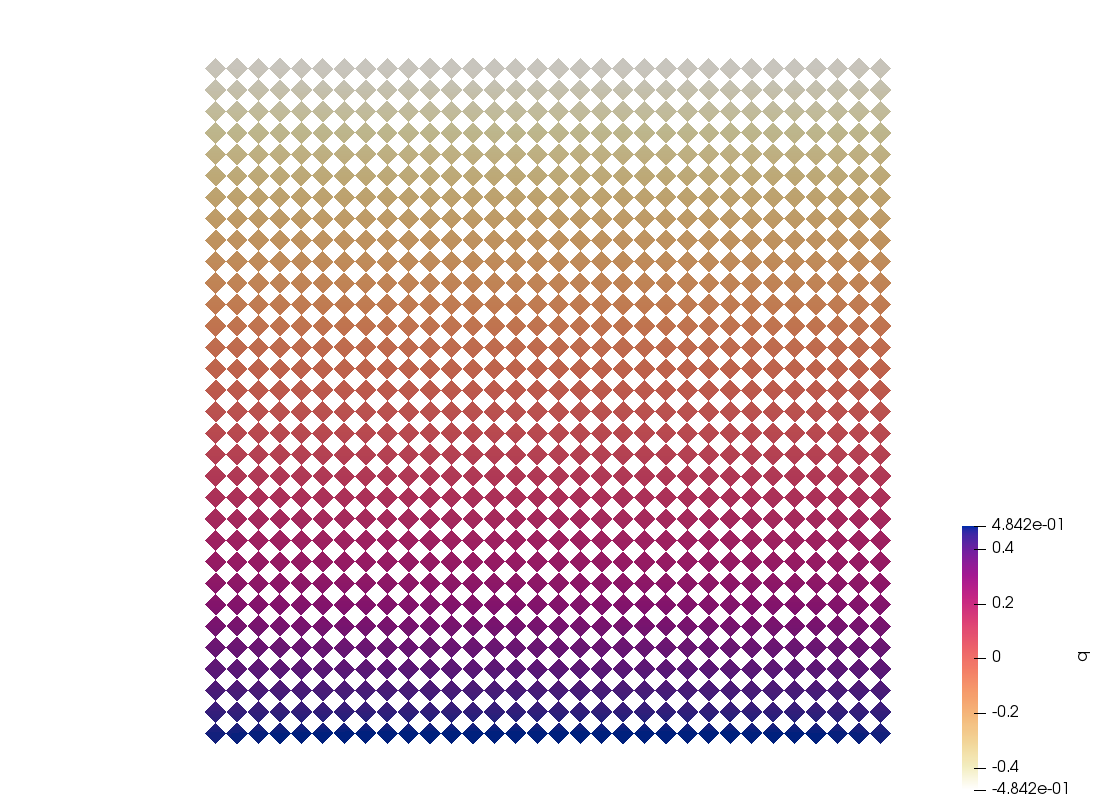
\includegraphics[width=4cm]{python_codes/fieldstone_77/results/block/pD}\\
{\captionfont From left to right: $\delta \rho=1,0.1,0.01,0.001$}

The conclusion is clear: in its current form, the element is not capable to 
deal with buoyancy-driven flows where $\delta \rho/\rho < 1\%$ which is 
unfortunately the type of simulations that are carried out in mantle dynamics modelling.
The reasons are (partially) discussed in Section~\ref{ss:RTq1p0}, but 
I am not sure how to go further. If an additional jump term is needed in the 
weak form in order to fix this problem, this makes the element not as simple as
advertised. 


%........................................................................
\subsubsection*{Another variant of a nonconforming quadrilateral element}

It is based on Han (1984) \cite{han84}.
The nodes are at the same location as for the RT element above, but 
there is an additional bubble function in the middle:
\begin{verbatim}
+====3====+
|         |
4    5    2
|         |
+====1====+
\end{verbatim}
Inside the reference element we assume that a field $f$
can be represented by 
\begin{eqnarray}
f^h(r,s) 
&=& a+ br +cs +d \phi(r) +e \phi(s) \\
&=& a+ br +cs +d \frac{5r^4-3r^2}{2}+e \frac{5s^4-3s^2}{2}
\end{eqnarray}
We then must have 
\begin{eqnarray}
f_1 = f^h(r=1,s=0) &=& a+ b +d \\
f_2 = f^h(r=0,s=1) &=& a+ c +e \\
f_3 = f^h(r=-1,s=0) &=& a- b +d \\
f_4 = f^h(r=0,s=-1) &=& a -c +e\\
f_5 = f^h(r=0,s=0) &=& a 
\end{eqnarray}
and we easily get 
\[
a = f_5 
\qquad
f_1-f_3 = 2b
\qquad 
f_2-f_4 = 2c
\]
followed by
\[
d=f_1-a-b = f_1 - f_5 - \frac{1}{2}(f_1-f_3) = \frac{f_1-2f_5+f_3}{2}
\]
and 
\[
e = f_2-a-c = f_2 - f_5 -  \frac{1}{2}(f_2-f_4) = \frac{f_2 -2f_5+f_4 }{2}
\]
Finally:
\[
f(r,s) = 
f_5 +
\frac{1}{2}(f_1-f_3) r+
\frac{1}{2}(f_2-f_4) s+
\frac{f_1-2f_5+f_3}{2} \phi(r)+
\frac{f_2 -2f_5+f_4 }{2} \phi(s)
\]
i.e.
\[
f(r,s) = 
\left(\frac{r + \phi(r)}{2} \right)f_1 +
\left(\frac{s+\phi(s)}{2} \right)f_2 +
\left(-\frac{r-\phi(r)}{2} \right)f_3 +
\left(-\frac{s - \phi(s)}{2} \right)f_4 +
\left(1-\phi(r)-\phi(s) \right)f_5 
\]
which has us define 
\begin{eqnarray}
N_1(r,s) &=& \frac{r + \phi(r)}{2} \\
N_2(r,s) &=& \frac{s+\phi(s)}{2}\\
N_3(r,s) &=& -\frac{r-\phi(r)}{2} \\
N_4(r,s) &=& -\frac{s - \phi(s)}{2}\\
N_5(r,s) &=& 1-\phi(r)-\phi(s)
\end{eqnarray}
We have of course the following properties $\sum_{i=1}^5 N_i(r,s) = 1$ and 
$N_i(r_j,s_j) = \delta_{ij}  \qquad i,j \in 1,5$. The partial derivatives of the shape functions are as follows
\begin{eqnarray}
\partial_r N_1(r,s) &=& \frac{1 + \phi'(r)}{2} \\
\partial_r N_2(r,s) &=& 0 \\
\partial_r N_3(r,s) &=& -\frac{1-\phi'(r)}{2} \\
\partial_r N_4(r,s) &=& 0 \\
\partial_r N_5(r,s) &=& -\phi'(r) \\
\partial_s N_1(r,s) &=& 0 \\
\partial_s N_2(r,s) &=& \frac{1 + \phi'(s)}{2} \\
\partial_s N_3(r,s) &=&  0 \\
\partial_s N_4(r,s) &=& -\frac{1-\phi'(s)}{2} \\
\partial_s N_5(r,s) &=& -\phi'(s)
\end{eqnarray}
This element is implemented in the {\tt stone\_han.py} file. 
Unfortunately it suffers from the exact same issue as mentioned above...






